\begin{abstract}
An OFDM structure from modulator to demodulator is studied. The aim is to investigate the characteristics of the system in different conditions and comparing the behavior with the single carrier configuration. The simulation conditions change in the cyclic prefix size, a Non-Linear Amplifier (NLA), multipath and equalizer activation. \\ Optimization on the cost function for the system is done. Semi-Analysis calculation for noise for a target Bit Error Rate (BER) of $10^{-3}$ are done. OFDM simulation is based on the characteristic of Fast Fourier Transform.\\
The analysis shows that using a multipath increases the needed \textit{energy per bit to noise power spectral density ratio} $(E_{b}/N_{0})$ by $13dB$ in order to reach the target BER when the NLA block is deactivated. An equalization block improves by $8dB$ the $(E_{b}/N_{0})$. In comparison, the multipath, more than the guard time of the signal, does not influence the BER so much.\\ With activated NLA with fixed $\beta=10$ the $E_{b}/N_{0}$ has to be amplified by almost $0.8dB$ in order to reach the target BER. \\ The optimized back-off of $\beta=8$ improves this value by $14dB$ when equalization block is activated.
 
\end{abstract}

\section{Introduction}
An OFDM communication system is simulated. Different characteristics of the system are examined and parameters are adjusted to study.\\ A block based signaling configuration is chosen for the implementation. As a result, the realization of the modulator is done thanks to IFFT computation characteristics. Cyclic prefixes are added to the resulting OFDM symbols as well as guard time filling. On the demodulator an FFT block recreates the initial input of the system. \\
An optimization is performed on the input back-off of a Non-Linear Amplifier (NLA). The back-off of the NLA is normally more than in a single carrier system because of better performance of the inter symbol interference (ISI) thanks to smaller coherent bandwidth which let us work on less power. \\
A description of the the system is given in section \ref{sec_systemmodel}. Section \ref{sec_simstruct} describes the varied parameters and analysis values while in section \ref{sec_anasim} observations on the simulation are presented and characteristics of the system are shown. Before the conclusion in section \ref{sec_conclusion}, section \ref{sec_optimization} describes the optimization of the system.

\section{System Model}
\label{sec_systemmodel}
\begin{figure}[tbp]
\centering
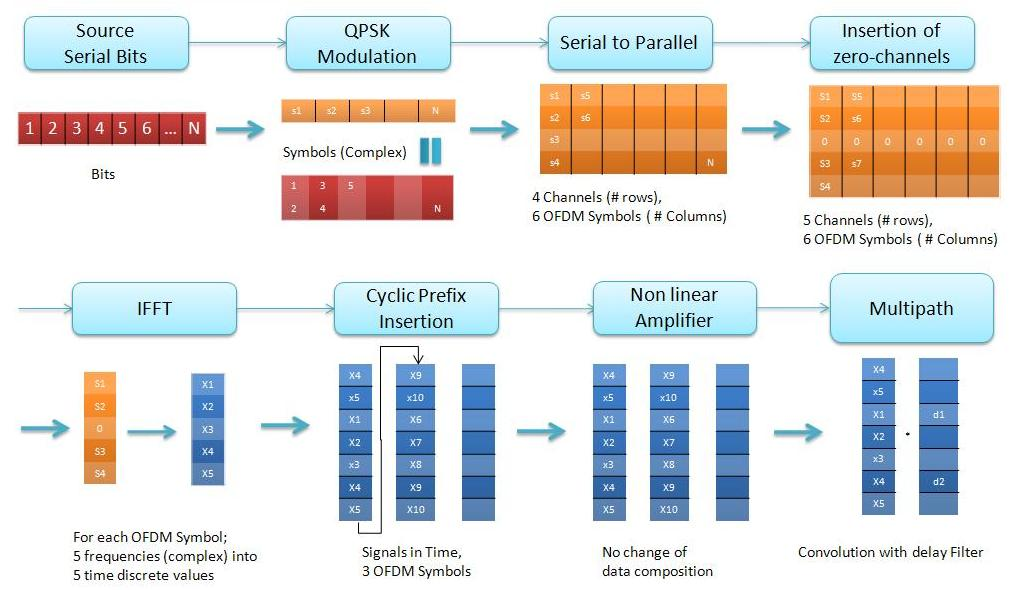
\includegraphics[width=\textwidth]{content/fig6/ofdmmodel1.JPG}
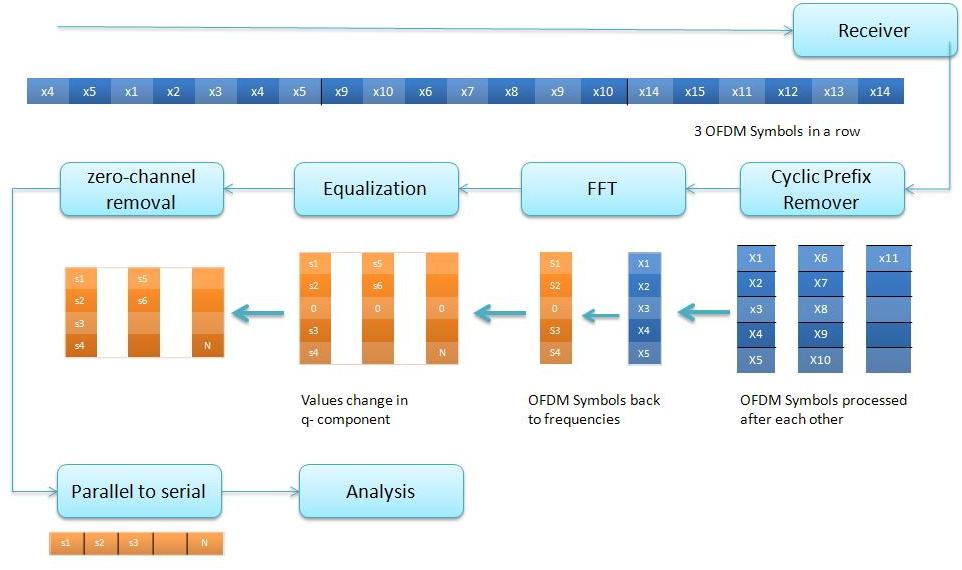
\includegraphics[width=\textwidth]{content/fig6/ofdmmodel2.JPG}
\caption{OFDM System Model}
\label{fig_ofdmsystemmodel}
\end{figure}

Figure \ref{fig_ofdmsystemmodel} presents the OFDM system block diagram.
Basic steps of the praxis are realized in blocks in the simulation. Additionally is shown how the composition of data changes in the single steps of the system.\\
The first block represents the data source. They are the bits which an application may send. In the simulation it is realized by a random bit generator. The following QPSK modulation block converts this bits into symbols, which are complex numbers. Each symbol carries several bits. The third block is the first one actually relevant for OFDM. The serial symbol stream is converted into a channel and OFDM symbol structure. In the simulation it is represented in a matrix shape where the rows are different channels and each column is an OFDM symbol. This means that each OFDM symbol, formed by $c$ (\#channels) serial symbols (complex numbers), is distributed over the $c$ channels.\\
In the next step zero channels are added in order to separate well subsequent OFDM symbols. For the simulation structure zero rows are added in the middle of the matrix. The following block interprets each symbol (complex number) of an OFDM symbol as a orthogonal frequency and converts each OFDM symbol per IFFT into a vector of time discrete values of the same length. As sixth step the cyclic prefix insertion is done. In order to maintain orthogonality of the frequencies but prevent ISI, an amount of \textit{guard values} are copied from the end of each OFDM symbol to its beginning. The number of rows in the simulation matrix grows by that by the number of \textit{guard values}.\\
The following block is the NLA which depends on the optimization parameter $\beta$ (back-off). At this point the transmitter side ends. In order to simulate the multipath a convolution is made on each OFDM symbol with the delay filter. Since the simulation is made on each OFDM symbol separated, this operation works with a memory in order simulate a serial transmission.\\
The receiver side is just the opposite of the transmitter. In the cyclic prefix remover the copied values are deleted and the simulation matrix size decreases. The next block performs the FFT on each OFDM symbol which reconstructs the as frequencies interpreted complex numbers.\\ The following equalization block tries to remove the effect of the multipath. For the simulation a multiplication with the inverted transfer function of the multipath is operated. By this, only the phase of the complex symbols changes.\\ Finally, the zero channels are removed and the matrix structure is reconverted to a series of symbols. The following analysis is done on the received symbols and consequently they are not demodulated into a bitstream.

\section{Simulation Structure}
\label{sec_simstruct}
Fundamentally, we do block-by-block simulation thanks to IFFT for parallel processing. Simulation is done by (de)activation of the blocks on Figure \ref{fig_ofdmsystemmodel}.
First, we study the noise semi-analysis by having only the basic blocks activated and also to examine the correctness of them. The basic blocks for our OFDM system are IFFT and FFT, Cyclic addition and removal and the semi-analyzer block. 
The theoretical equation of the BER for a QPSK channel is:\\
\begin{center} 
$P_{b}(e)= \frac{1}{2}erfc(\sqrt{\frac{E_{b}}{N_{0}}})$\\
\end{center}
It is discussed that the BER can be computed by considering the non-ideality which the two parameters \textit{guard time} and \textit{pilots} will inject into the result. The formulation would be:\\
\begin{center}
 $P_{b}(e)= \frac{1}{2}erfc(\sqrt{\frac{E_{b}}{N_{0}}\frac{T}{T+T_{g}}\frac{N_{u}}{N_{u}+N_{p}}})$\\
\end{center}

In the next step, the NLA block is activated and its effect is studied. We have chosen NLA number 3 and try to optimize its back-off.
Later, the channel impulse response modeled by considering two multipaths with different delays is implemented by an FIR filter. This extended simulation will be compared with NLA in the scenario and also the equalizer. Finally, we optimize the system by adjusting the back-off parameter of NLA in an AWGN channel.\\
When we study the equalization block we consider such equation for the received tones:
\begin{center}
$y_{i}= H_{i} \lambda_{i} + n_{i}$\\
\end{center}
Without equalization the BER would be:
\begin{center}
$P_{b}(e)= \frac{1}{2}erfc(\frac{H_{i} \lambda_{i}}{\sqrt{2 \sigma^{2}}})$\\
\end{center}
Then, after the equalization, the formula will be changed to this:\\
\begin{center}
$y^{\prime}_{i}= \lambda_{i} + \frac{n_{i}}{H_{i}}$\\
\end{center}
and the BER to
\begin{center}
 $P_{b}(e)= \frac{1}{2}erfc(\frac{\lambda_{i}}{\sqrt{2 \sigma^{2}}})$\\
\end{center}
and NOT: $P_{b}(e)= \frac{1}{2}erfc(\frac{\lambda_{i}}{\sqrt{\frac{2 \sigma^{2}}{H_{i}}}})$, as it may be guessed wrongly. The power spectral density of the noise is not decreased.
\section{System Design in System Generator}
\label{sec_anasim}

Then main core of an an OFDM modulator and demodulator are the inverse FFT (IFFT) and FFT respectively. In 802.11a WLAN standard a 64-point transform with 52 of the subcarriers are carrying user data in a BPSK,
QPSK, 16-QAM or 64-QAM alphabet. The symbol rate in this systems is $20 MSym/s$. The OFDM symbol period
is $4 \mu s$, with $3.2 \mu s$ of this interval occupied by the 64-point FFT symbol and the additional $0.8 ps$ used for the cyclic prefix.\\

The synchronization tasks is challenging in an OFDM-based communication system. Prior to performing channel estimation equalization and demodulation, OFDM symbol timing must be detected. The receiver has no information when a packet starts, and so the first synchronization task is packet detection. Once a packet has been detected the remaining synchronization functions include coarse and fine timing recovery and carrier recovery.\\
Figure \ref{ieee_preamble} shows the structure of the IEEE 802.1 la standard preamble. The 10 short preambles ($A_{1}$-$A_{10}$) are identical 16- sample duration sequences. The cyclic prefix (CP) is a 32- sample sequence and the long preambles ($C_{1}$ and $C_{2}$) are identical 64-sample sequences. As indicated in the figure, the various fields are used for packet detection, automatic gain control (AGC), diversity selection, coarse and fine frequency offset estimation, fine symbol timing estimation and channel estimation. 

\begin{center}
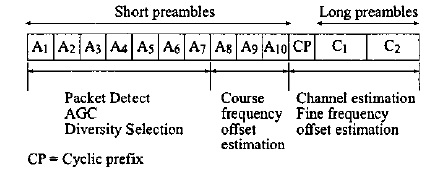
\includegraphics[width=\textwidth]{content/fig/ieee_preamble.JPG}
\captionof{figure}{IEEE 802.11a preamble.}
\label{ieee_preamble}
\end{center}


Figure \ref{ofdm_system} shows the main scheme of an OFDM system in transmitter and receiver. Another block of Channel is a Additive White Gaussian Noise which is used in simulation only.\\
As you can see there are some others blocks which are necessary for system implementations. The whole system is connected to a main hard processor which is located in the FPGA. It is a ARM Cortex-A9 with maximum frequency of $666.66 MHz$. EDK processor represents the main processor which connected to the OFDM block by AXI protocol. 

\begin{center}
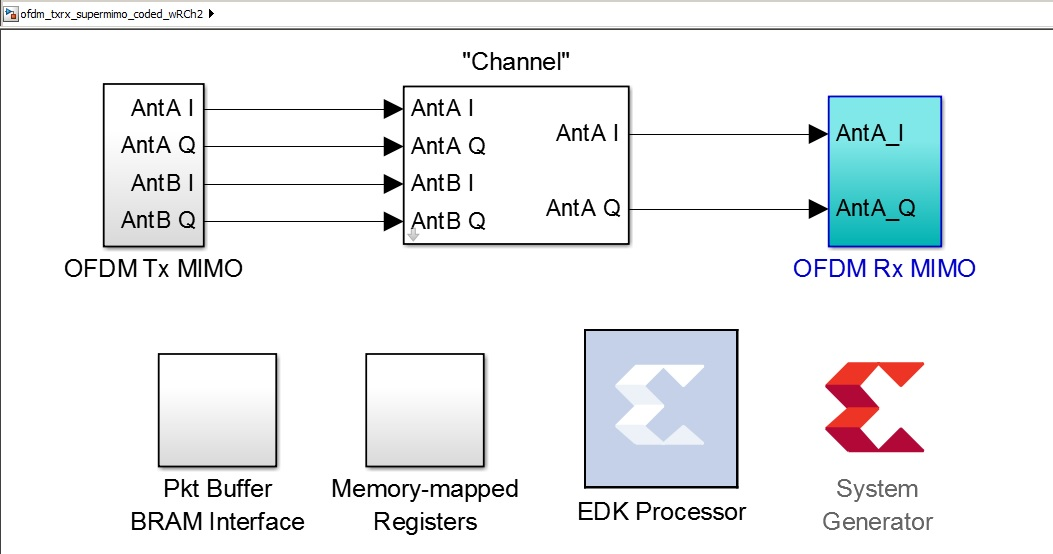
\includegraphics[width=\textwidth]{content/fig/system.JPG}
\captionof{figure}{OFDM System.}
\label{ofdm_system}
\end{center}

Figure \ref{tx_block} illustrates the transmitter which consists of many blocks. Controlling of the time we have \textit{TxControl} block for synchronization of the blocks. It also generate the semi-fixed preamble (LTS and STS) and the relevant Training signals for the system. \textit{Training Data} generates the training pattern which is used to estimate the channel frequency response.
The main clock is IFFT which convert the time-based signals into frequency. In the current picture we set a 64 point IFFT although the recent design it upgraded to 256 as a result of the strategy changes. The data captured by the IFFT blocks are integrated in the \textit{OutputBuffers}. \textit{OutputMuxes} block chooses between two possible antenna to transmit the stream. In \textit{PreSpin, Filters DACs}, some sub-blocks for soft gain and DAC preparation data are implemented. Besides, the are a generic block to rate change matter which can be activated by the processor.\\

\begin{center}
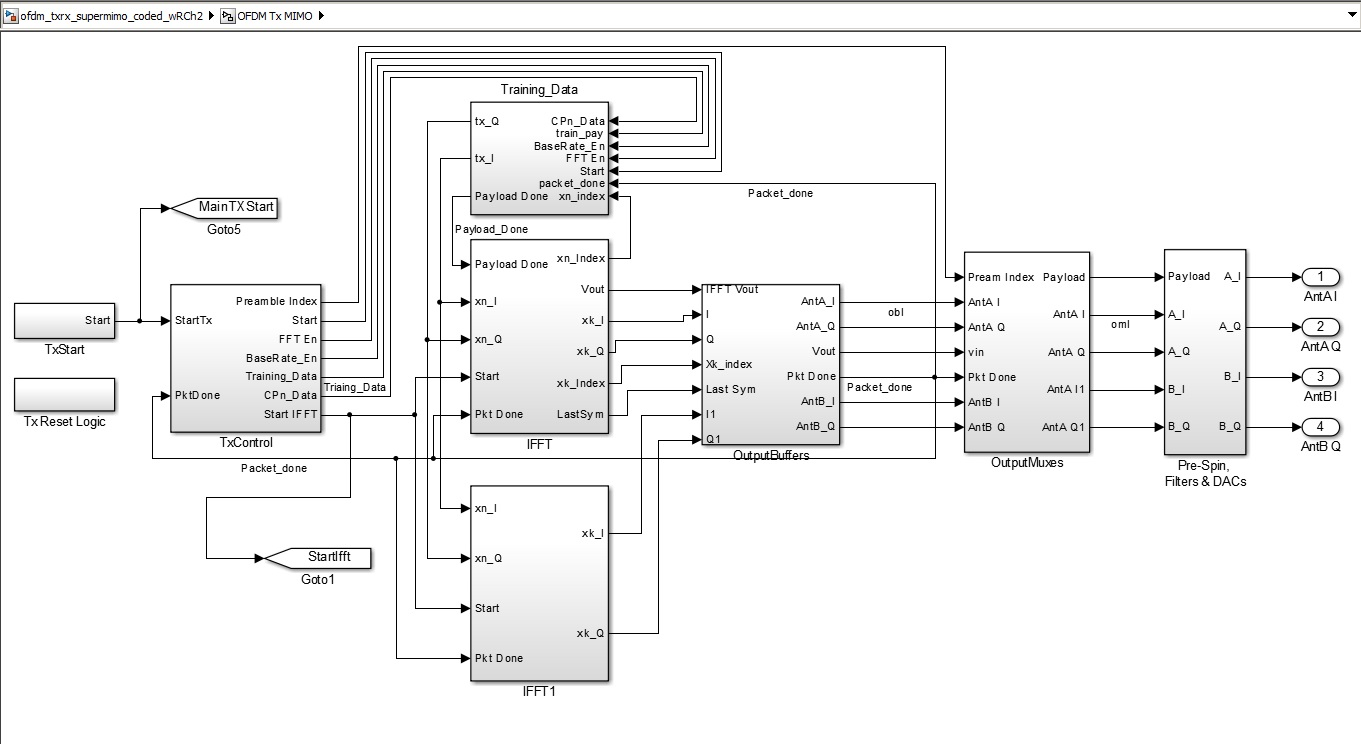
\includegraphics[width=\textwidth]{content/fig/txblock.JPG}
\captionof{figure}{OFDM Transmitter Block.}
\label{tx_block}
\end{center}

Figure \ref{rx_block} demonstrates the receiver block with its main blocks. The input signals enter into the device in a I/Q form from the analogue board. The is \textit{ADC inputs Antenna Selection} which we can switch between the two antennas and also the internal TX block which is reside in to the FPGA for the testing purposes. This block also adjust the input gain for the rest of the design. The frequency correction is done in the \textit{Coarse Freq Correction} using the STS stream.  
\begin{center}
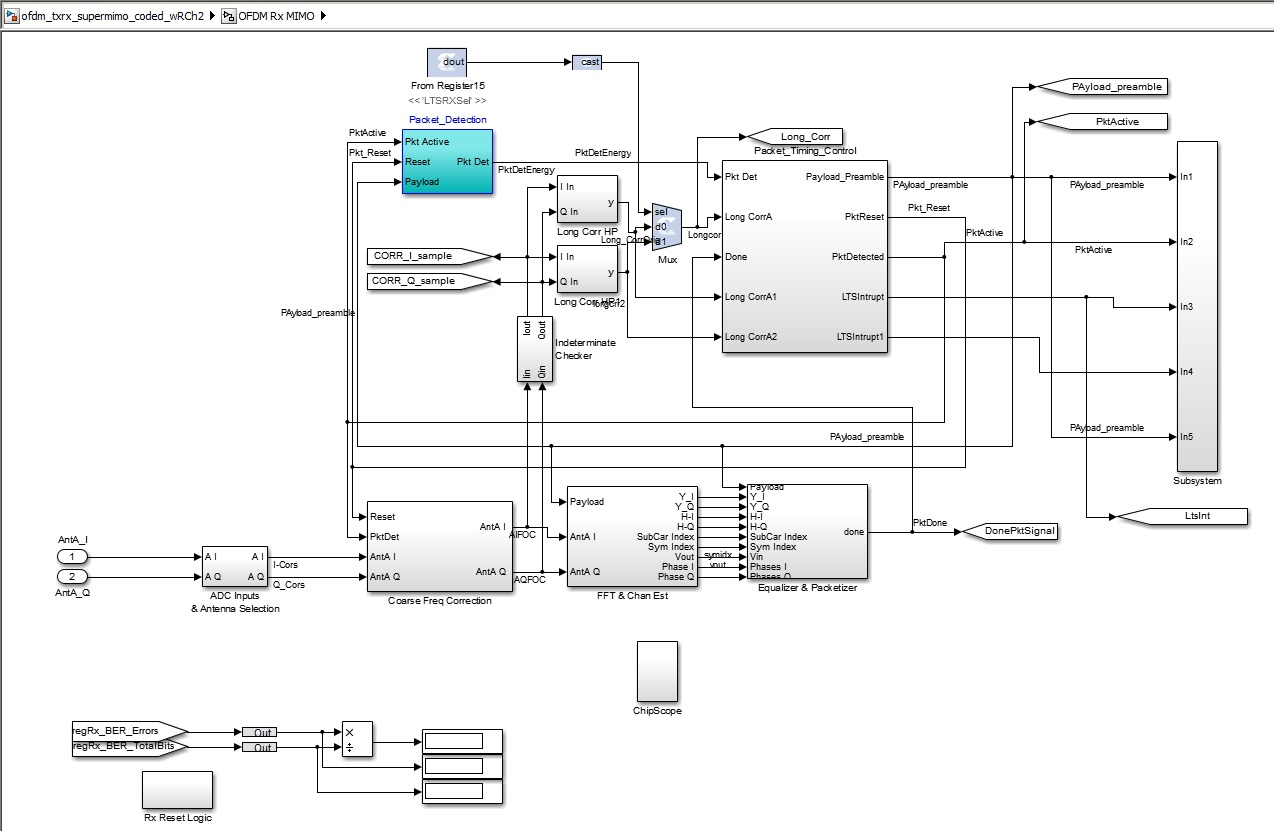
\includegraphics[width=\textwidth]{content/fig/rxblock.JPG}
\captionof{figure}{OFDM Receiver Block.}
\label{rx_block}
\end{center}

The packet detector is based on the Schimdl and Cox delay and correlate algorithm employed for acquiring symbol timing commonly. The algorithm, as illustrated in Figure \ref{schimdl_cox}, is basically a sliding window correlator combined with an energy detector used to normalize the decision statistic and hence guard against fluctuations of the input signal power level.\\

The sliding window P computes a auto-correlation between the input signal and a D-sample delayed version on short preamble interval. We chose D=16. The second sliding window R is used to compute the received signal energy in the cross-correlation interval. The cross-correlation P(n) and auto-correlation R(n) are calculated according to Eq. (I) and Eq. (2) respectively.\\

$ P(n) = \sum\limits_{m=0}^{L-1} r_{n+m} r^{*}_{n+m+D} $\\

$ R(n) = \sum\limits_{m=0}^{L-1} r_{n+m+D} r^{*}_{n+m+D} $\\

The decision statistic is computed as\\
$ M(n)= \dfrac{|P(n)|^{2}}{R(n)^{2}}$



\begin{center}
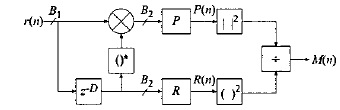
\includegraphics[width=\textwidth]{content/fig/schimdl_cox.JPG}
\captionof{figure}{Auto-Correlation Block.}
\label{schimdl_cox}
\end{center}

In the \textit{Packet Detection} block an auto-correlation approach is done on the signal to detect the energy of the preamble in the beginning of STS shows in Figure \ref{autocorrblock}. This is implemented based on the magnitude square of the both I/Q signals and comparing with a threshold after a sliding window. In other branch a multiplication of of the imaginary and real part with their 16 clock delayed version is calculated and the square magnitude in a sliding windows is detected. In \textit{Detection Decision} we use some other threshold to be ensure if the two cross correlation peaks are detected in the right time to signal the packet detection.

\begin{center}
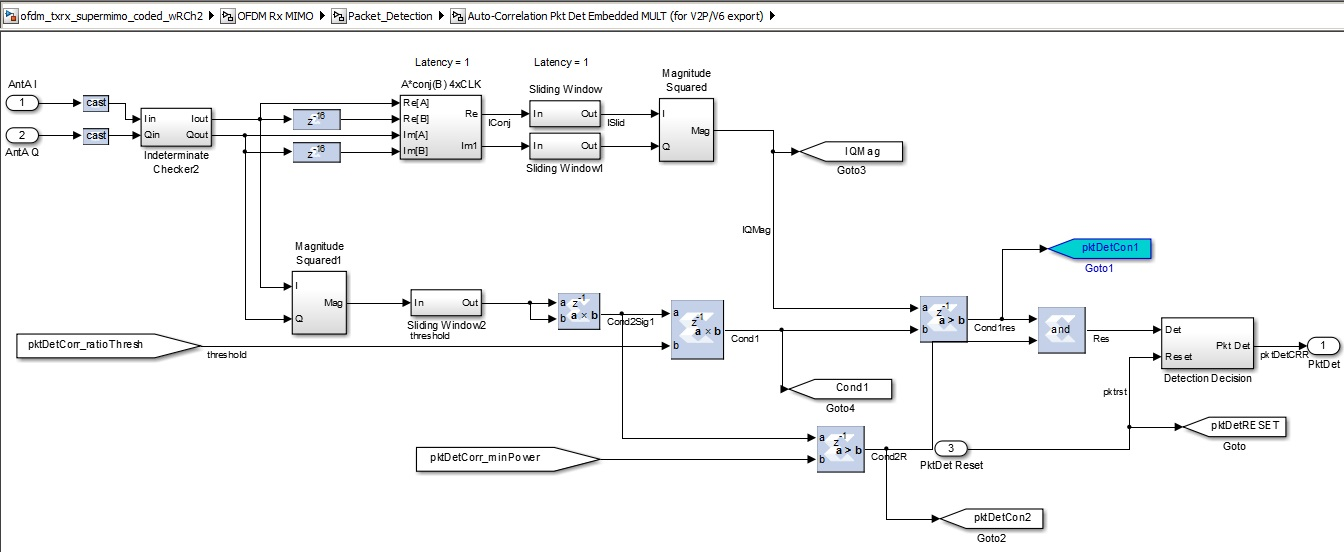
\includegraphics[width=\textwidth]{content/fig/autocorrblock.JPG}
\captionof{figure}{Auto-Correlation Block.}
\label{autocorrblock}
\end{center}

\begin{center}
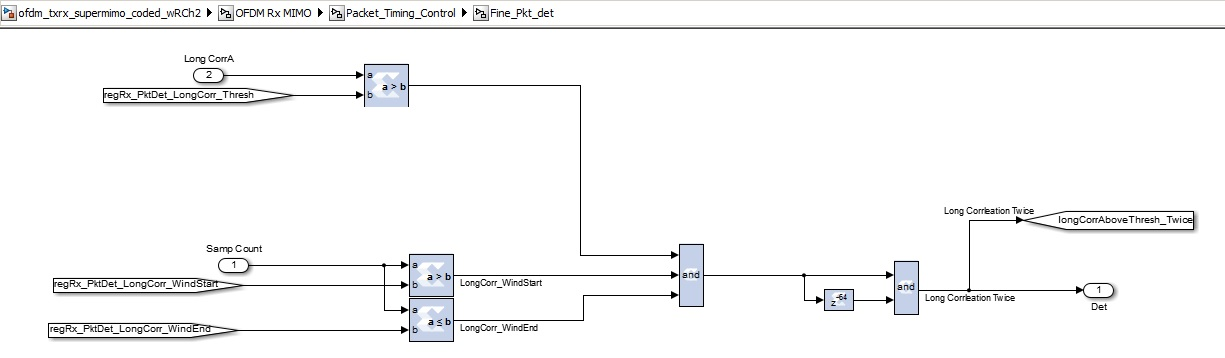
\includegraphics[width=\textwidth]{content/fig/fine_packetDetect.JPG}
\captionof{figure}{Fine Packet Detection Block.}
\label{autocorrblock}
\end{center}

\section{Hardware Samples and Analysis}
\label{hw_samples}

\begin{center}
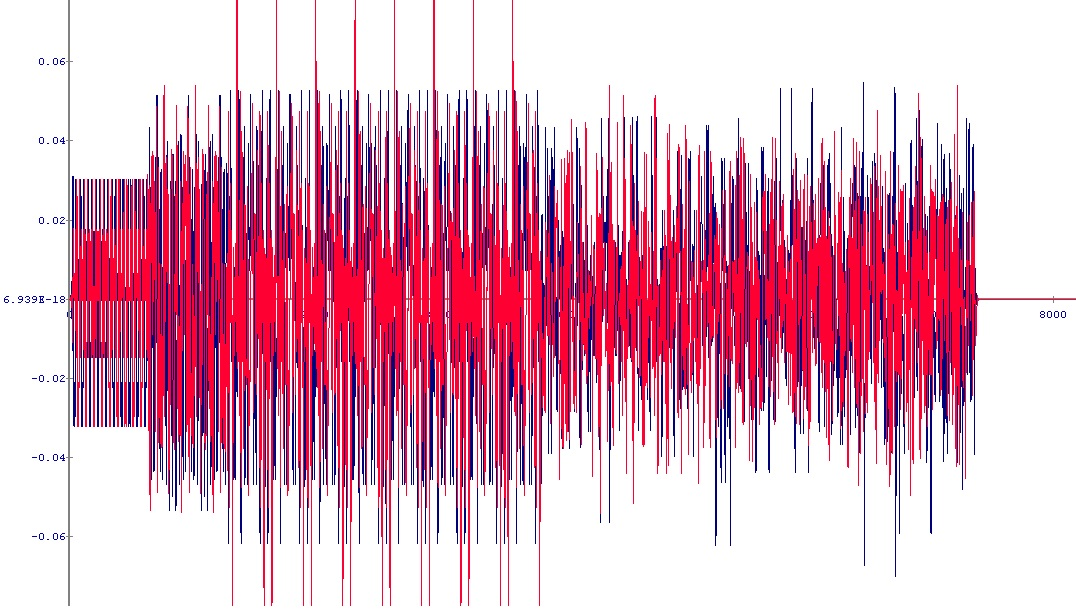
\includegraphics[width=\textwidth]{content/fig/ofdmframe_chipscope.JPG}
\captionof{figure}{OFDM Frame (I/Q) detected in Chipscope.}
\label{ofdmframe_chipscope}
\end{center}

\begin{center}
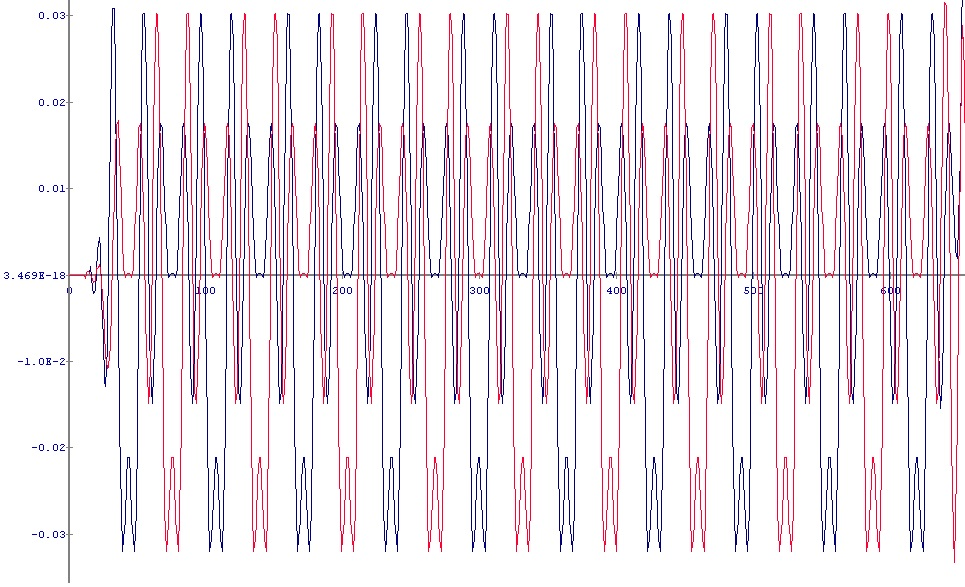
\includegraphics[width=\textwidth]{content/fig/sts_chipscope.JPG}
\captionof{figure}{STS (I/Q) detected in Chipscope.}
\label{sts_chipscope}
\end{center}

\begin{center}
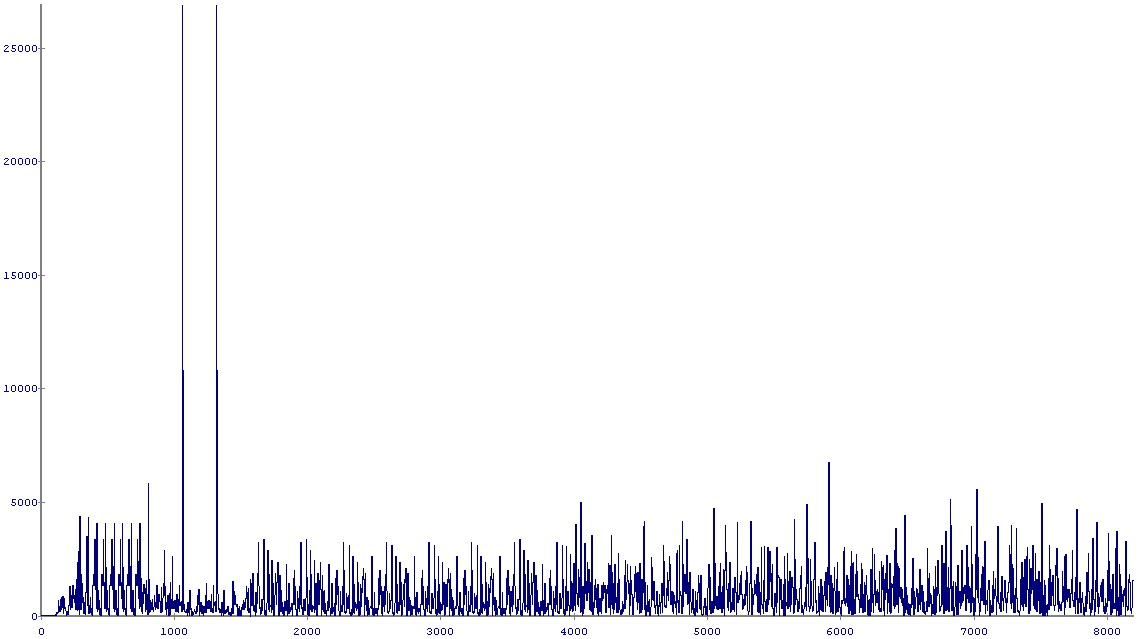
\includegraphics[width=\textwidth]{content/fig/crosscorr.JPG}
\captionof{figure}{Cross-Correlation detected in Chipscope.}
\label{crosscorr}
\end{center}


\begin{center}
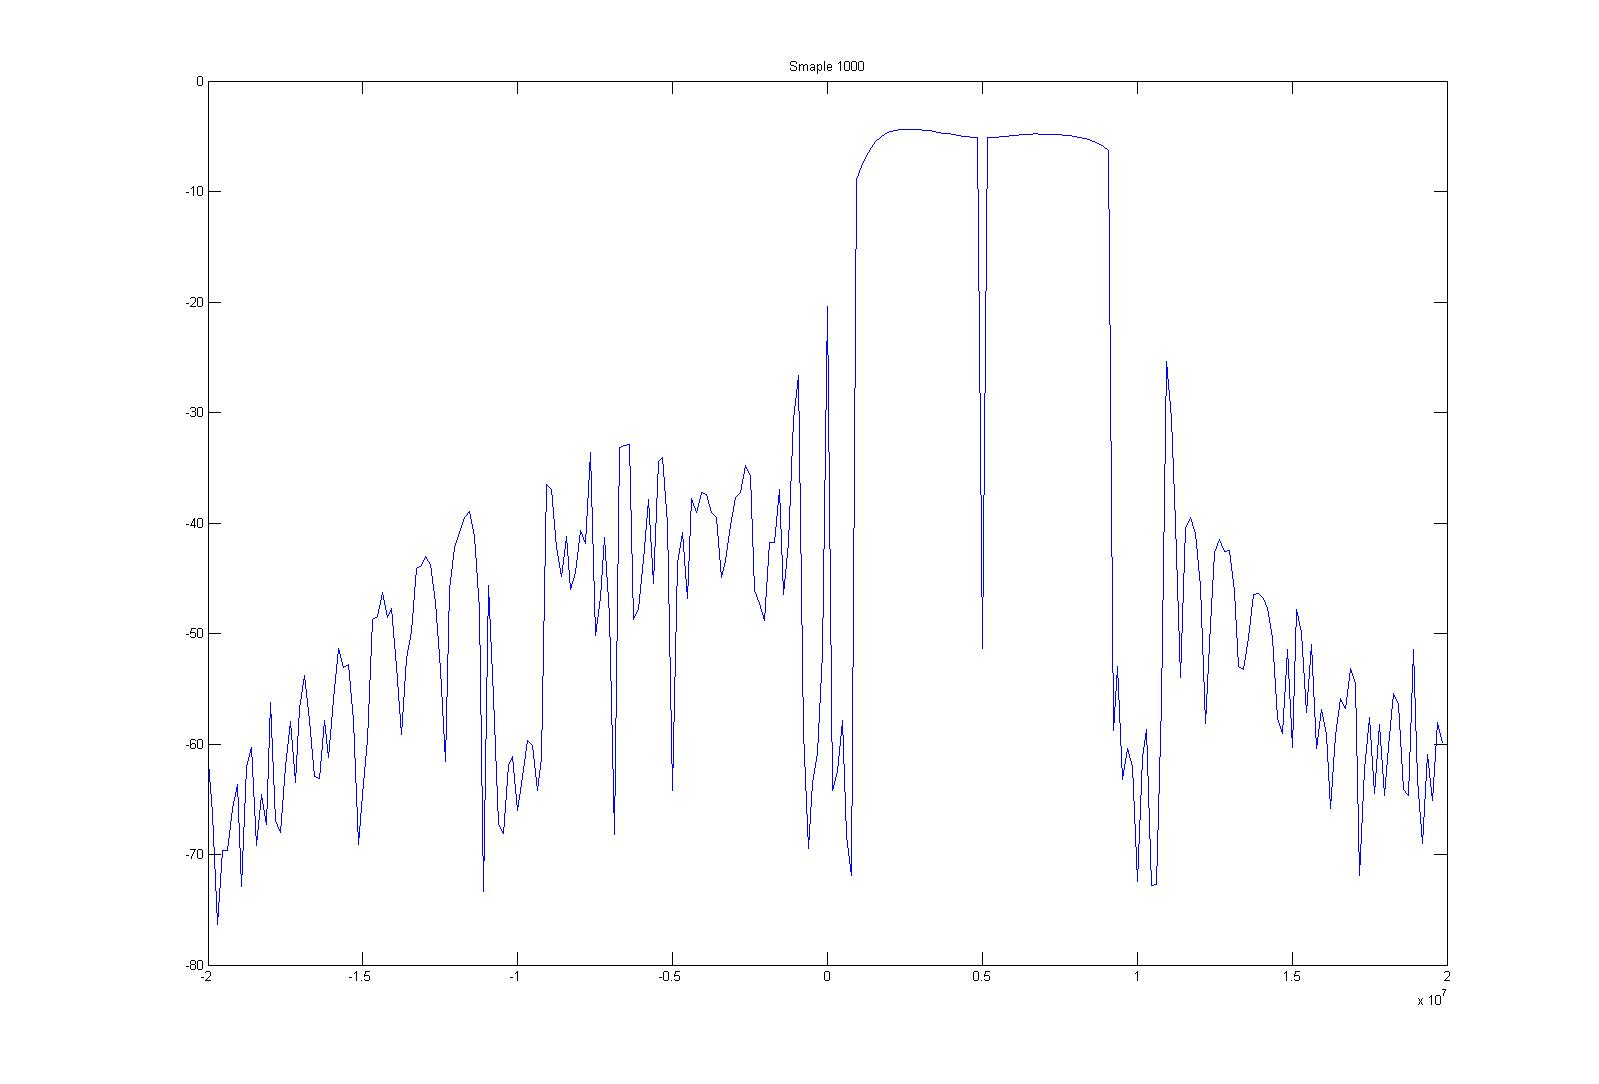
\includegraphics[width=\textwidth]{content/fig/baseIFAdcDac.JPG}
\captionof{figure}{LTS Spectrum in Baseband chain (IF filter is enable)}
\label{baseIFAdcDac}
\end{center}

\begin{center}
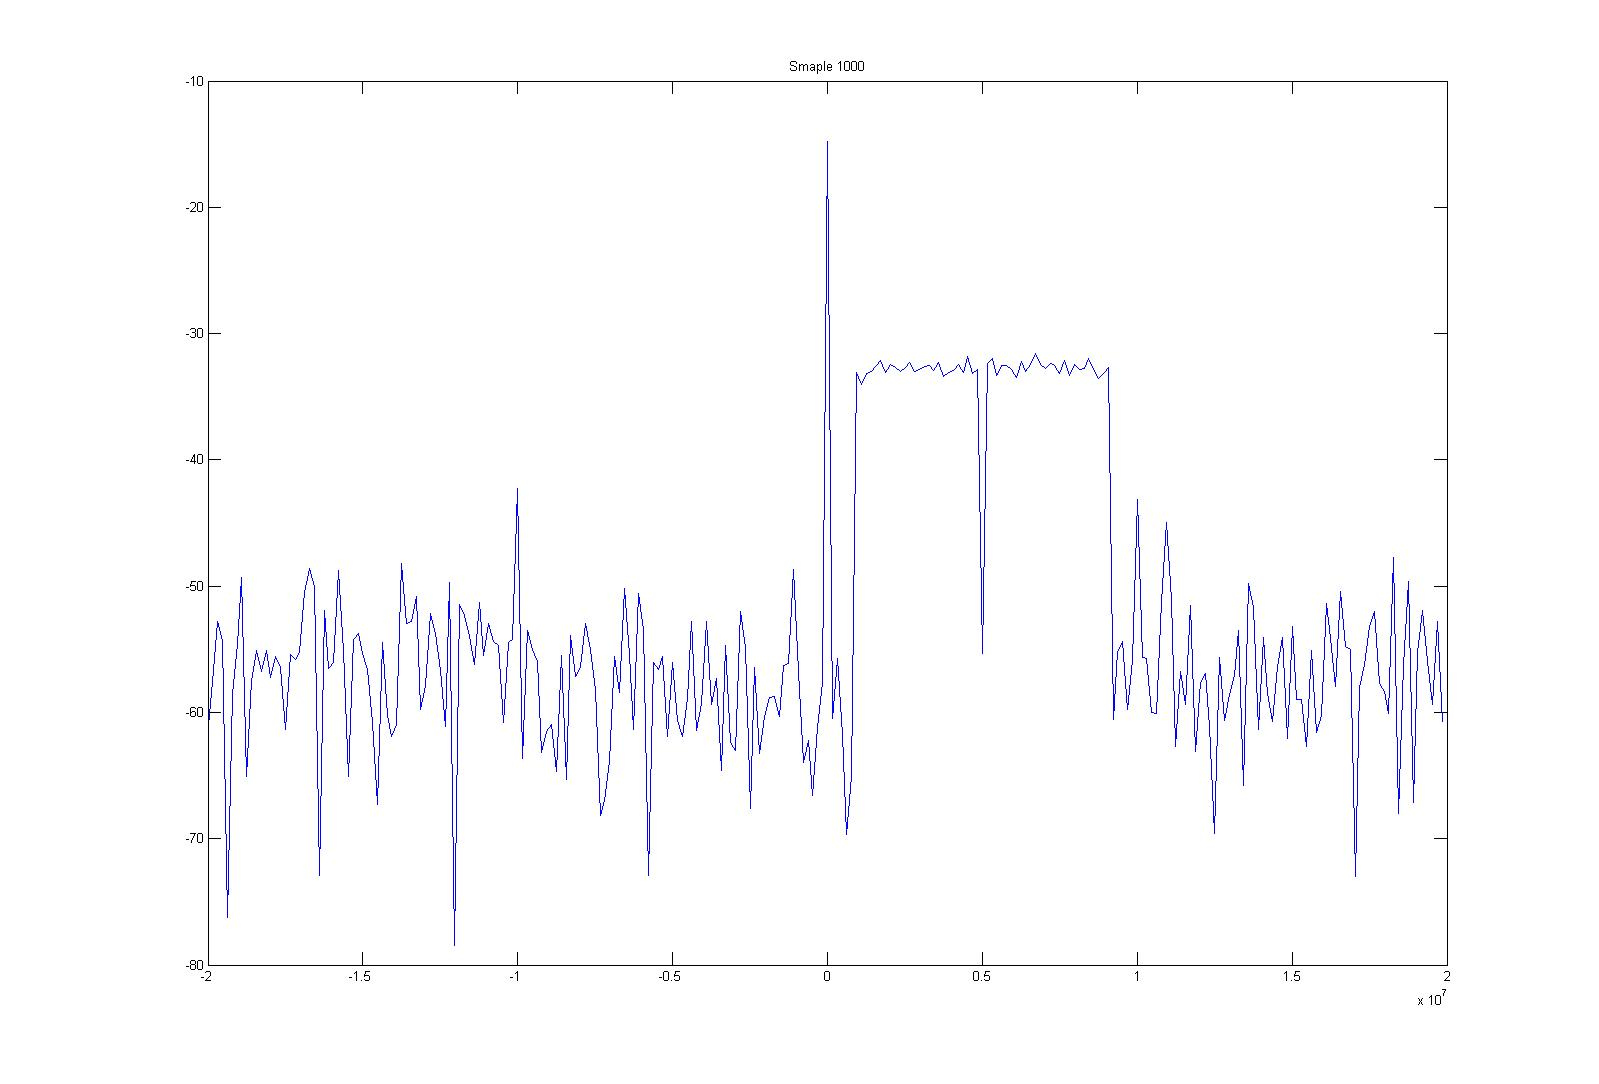
\includegraphics[width=\textwidth]{content/fig/RfIF.JPG}
\captionof{figure}{LTS Spectrum- passed RF chain (IF filter is enable)}
\label{RfIF}
\end{center}

\begin{center}
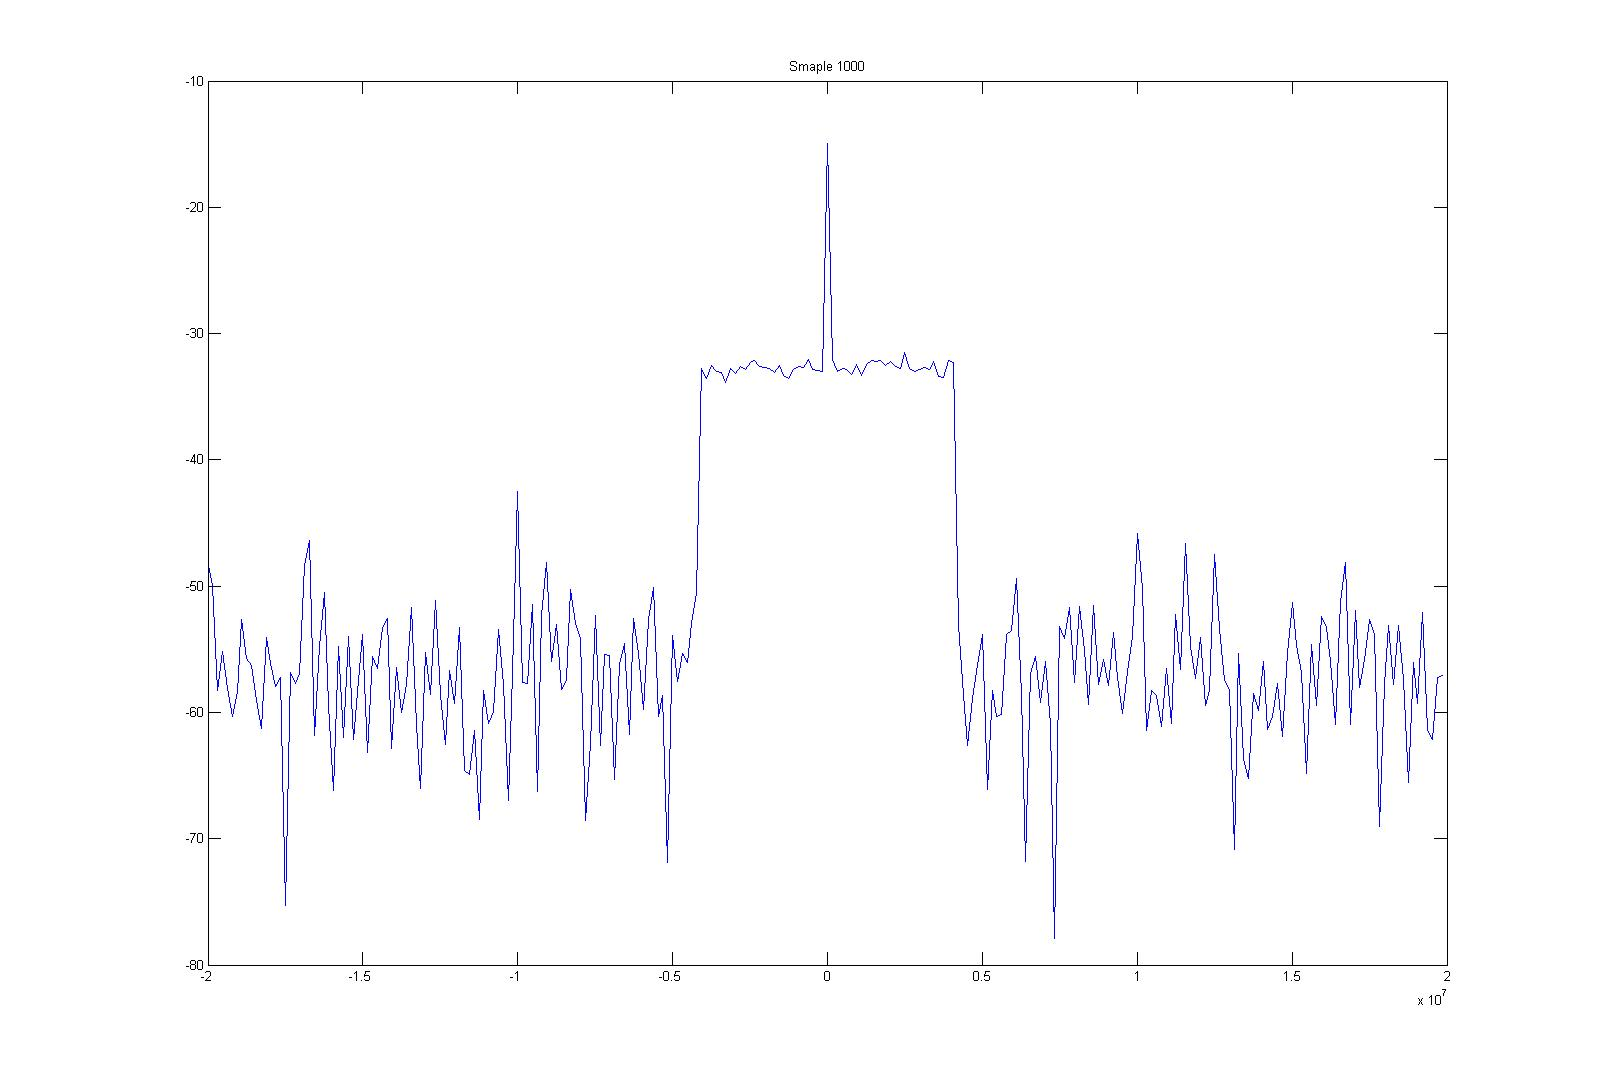
\includegraphics[width=\textwidth]{content/fig/Rfbase.JPG}
\captionof{figure}{LTS Spectrum- passed RF chain (IF filter is disable)}
\label{Rfbase}
\end{center}

\begin{center}
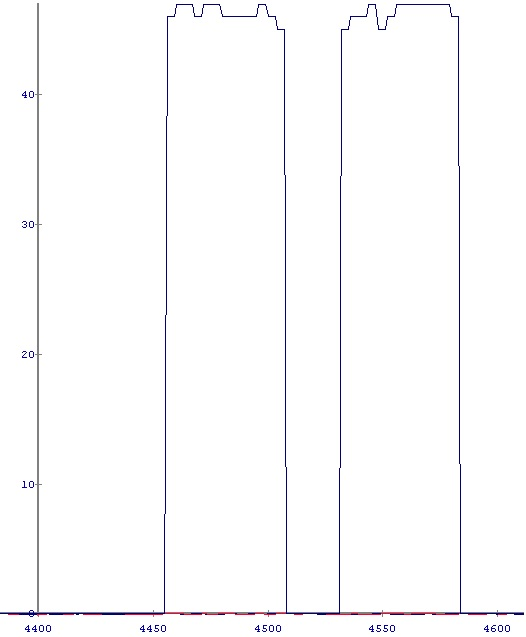
\includegraphics[width=\textwidth]{content/fig/h_mag_chipscope.JPG}
\captionof{figure}{Frequency Response of a semi-perfect channel detected in Chipscope}
\label{h_mag_chipscope}
\end{center}

\section{FPGA Inside}
Based on the Xilinx All programmable SoC architecture, the Zynq-7000 All Programmable SoCs enable extensive system level differentiation, integration, and flexibility through hardware, software, and I/O programmability. Using the Zynq-7000 platform, you can design smarter systems with tightly coupled software based control and analytic with real time hardware-based processing and optimized system interfaces.\\
As you can see in Figure \ref{zynq_inside} the foundation of Zynq-7000 is divided into two main parts. Firstly, Processor System which are two ARM processors and the fixed implemented peripherals. The rest are just the raw Programmable Logic which the main OFDM physical layer is implemented inside. We should build the gates, DSP and RAM in this region by VHDL programming or System Generator software in Matlab environment.\\


\begin{center}
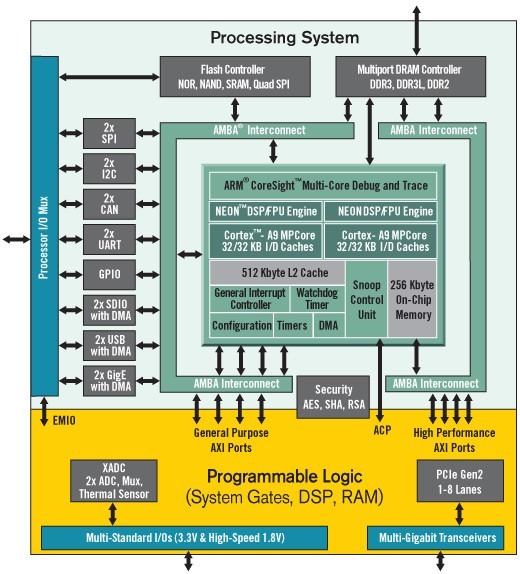
\includegraphics[width=\textwidth]{content/fig/zynq_inside.JPG}
\captionof{figure}{Zynq-7000 Diagram}
\label{zynq_inside}
\end{center}

The block diagram of the design is illustrated in Figure \ref{design_block_diagram}. We activate one of the ARM processors. In the TX chain, a PC sends a packet data via the Ethernet port to Zynq-7000. The EMAC block receives the packet and DMA it into the RX Block RAM which is divided into $32$ bank with size of $2K \times 64-bit$ which realize a Circular Buffer to relief the burst data stream enters from the asynchronous Ethernet port. As the OFDM block works in $40 MHz$ and each $2K$ block reading takes maximum $50\mu s$ for the EMAC and OFDM-PHY pessimistically, the tolerance of the Ethernet stream will be $\frac{32 \times \ 64b}{50\mu s} = 40Mbps$ which proves good number of banks. The offset pointer of reading and writing by DMA MAC which is govern under a scatter-gather scheme and the OFDM-PHY is controlled by the ARM.\\

\begin{center}
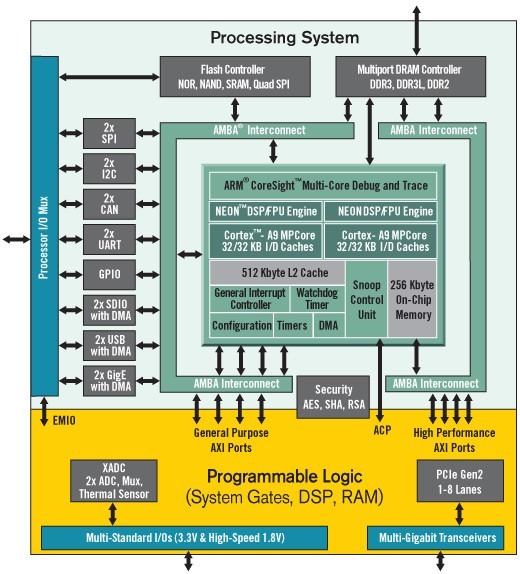
\includegraphics[width=\textwidth]{content/fig/zynq_inside.JPG}
\captionof{figure}{Design Block Diagram}
\label{design_block_diagram}
\end{center}

As you can see in the block diagram the connection bridge between the Processor System and the Programmable Logic in the Zynq architecture can be AXI protocol. You can find the detail of AXI at ref..... There are some other communication protocols but in the Zynq design AXI works optimum.
For easier programming issues in PC side, we used Linux Virtual Machine inside a Windows OS. It is very helpful because this configuration prevents unnecessary data exchange of the system and helps us to have a real estimation of the bit rate.\\

\section{Step-by-step Design}
The configuration set-up is consisted of two Zynq board each carrying a FMCOMMS1 radio board. They are connected to two individual PC via Ethernet cables as shown in Figure \ref{hardware_setup}.\\

\begin{center}
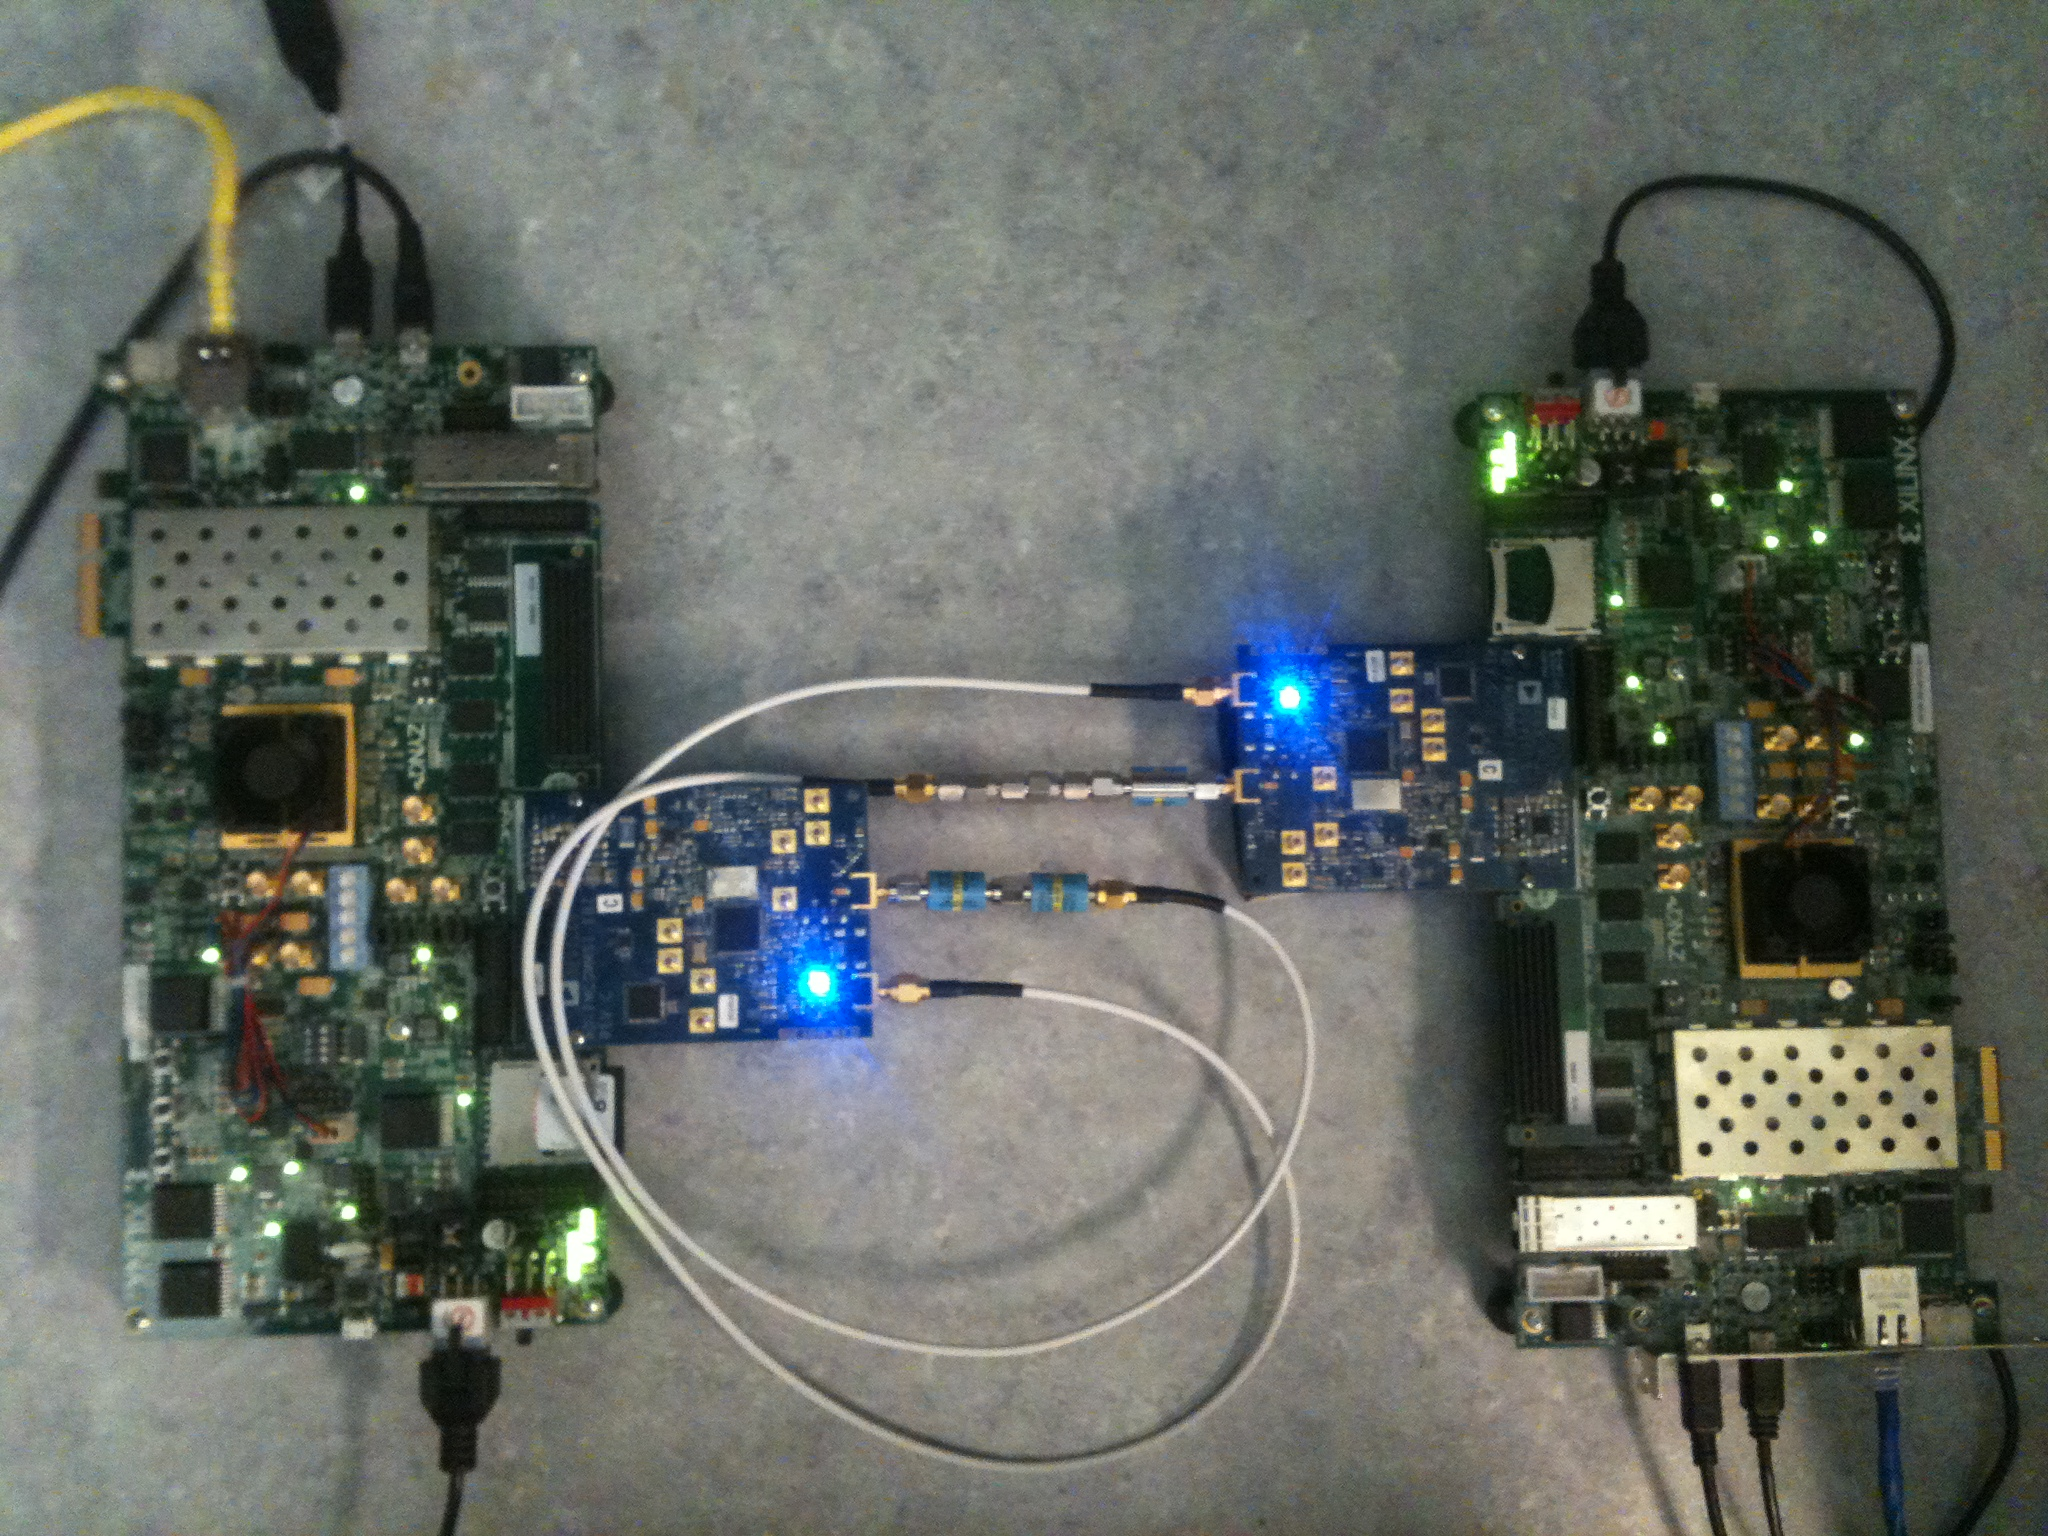
\includegraphics[width=\textwidth]{content/fig/hardware_setup.JPG}
\captionof{figure}{Hardware set-up}
\label{hardware_setup}
\end{center}

This configuration should be tested partially and have realistic estimation of the maximum possible bit-rate and then calculate SNR of channel. Having engineering steps to examine each hardware block, we check the loops illustrated in \ref{design_block_diagram}.\\
The maximum bit rate we could reach to exchange via Ethernet peripheral of the Zynq board which is called EMAC is $600 Mbps$. This was a time consuming task to reach to this bit rate considering the complicated Direct Memory Access mechanism implemented in near contact of EMAC inside of ARM processor. Fortunately, there were many useful application examples dedicated by Xilinx but still it should study many document to understand the scheme in RX and TX of Ethernet.\\
Next, the correct configuration of the two TX and RX BRAMs are checked by directly data replacement between the two banks specified by the ARM processor. This was an important step because the maximum data rate is very depends on the correct data reading and writing into these two blocks. There is an useful functionality of the RAM which is designed also in Zynq-7000 that called Error-Correction Code (ECC). This is a type of computer data storage that can detect and correct the most common kinds of internal data corruption. ECC memory is used in most computers where data corruption cannot be tolerated under any circumstances, such as for scientific or financial computing. The two BRAMs communicate with AXI Bus via an BRAM controllers. The configuration of the BRAMs and the controllers should be set accordingly.\\
The main part of the project is dedicated of the OFDM-PHY block with its sophisticated details.\\

